\subsection{Motivation}

First introduced by Ying and coworkers \cite{Ying:2004:JCP}, the kernel-independent FMM (\textbf{\gls{KIFMM}})
provides an algorithm, that maintains the basic recursive structure and $O(N)$
asymptotic complexity of the analytic FMM, but without the requirement for the
implementation of analytic expansions of the kernel function for each kernel.
Instead the method relies only on kernel function evaluations. This allows
software implementations to be written in an easily extensible manner for different
kernels. The main difference to the analytic FMM of Section \ref{sec:1_1_fmm_overview},
lies in the the way that source and target densities are represented, and how
the M2M, L2L and M2L operators are computed.

\subsection{Algorithm Structure \& Analysis}

For the \gls{KIFMM} presented in \cite{Ying:2004:JCP} the \gls{far-field}, $\mathcal{F}^B$, and
\gls{near-field}, $\mathcal{N}^B$, have precise specifications. For a given box $B$
centered at $\mathbf{c}$ with sides of length 2$r$, $\mathcal{N}^B$ is a box
centered at $\mathbf{c}$ with sides of length 6$r$. The \gls{far-field} is then
defined as $\mathbb{R}^d / \mathcal{N}^B$, where $d$ is spatial dimension.
Here, $B$ is in the \gls{near-field}. Consider the potential in the \gls{far-field} $\mathcal{F}^B$, generated by a
set of \gls{source-particles}, described by \textbf{\gls{source-densities}}
$\{\phi_i, \> i \in I^B_s \}$ where $I^B_s$ is the set of indices for the \gls{source-particles}
in box $B$\footnote{This notation matches that used in \cite{Ying:2004:JCP}
in order for ease of reference.}. Specifying the indices for the \gls{source-particles}
specifically to make it clear that they may be distinct from the \gls{target-particles}.
These \gls{source-particles} can be equivalently described with an \textbf{upward \gls{equivalent-density}}
distribution $\phi^{B,u}$ supported at discrete points on an \textbf{upward \gls{equivalent-surface}}
$\mathbf{y}^{B, u}$ that encloses the set of source particles. The KIFMM relies
on the assumption that the potential produced by the equivalent densities is smooth,
which is guaranteed in the case that $\mathbf{y}^{B,u}$ does not overlap with the
far-field $\mathcal{F}^B$ \cite{Ying:2004:JCP}, furthermore the requirement that
$\mathbf{y}^{B,u}$ must enclose all particles in $B$ leads to the requirement
that it must also not overlap with $B$. For second-order linear elliptic
\textbf{\gls{PDE}}s, for which the KIFMM is defined,
and of which equation (\ref{eq:poisson}) is an example, the solution for the
potential in the far field, which can be seen as an exterior Dirichlet problem,
is guaranteed to be unique \cite{Ying:2004:JCP}. Therefore, the potentials
induced by the source particles and the equivalent densities satisfy are
guaranteed to be equivalent in the far field $\mathcal{F}^B$ if they coincide
at the boundary of the far field $\mathcal{F}^B$, or anywhere between the boundary
of the far field and the upward \gls{equivalent-surface}. This boundary is referred to
as the \textbf{upward \gls{check-surface}}, $\mathbf{x}^{B, u}$, and the entire
scheme is illustrated in figure (\ref{fig:1_2_upward_downward_surfaces}A).
The equality of the potentials from the source points and the equivalent density
can be stated mathematically as follows,

\begin{equation}
\int_{\mathbf{y}^{B,u}} K(\mathbf{x}, \mathbf{y})\phi^{B, u} d\mathbf{y} = \sum_{i \in I_s^B} K(\mathbf{x}, \mathbf{y})\phi_i = q^{B, u} \> \> \text{for any} \> \> \mathbf{x} \in \mathbf{x}^{B, u}
\label{eq:1_2_p2m}
\end{equation}

\begin{figure}[!h]
    \centering
    {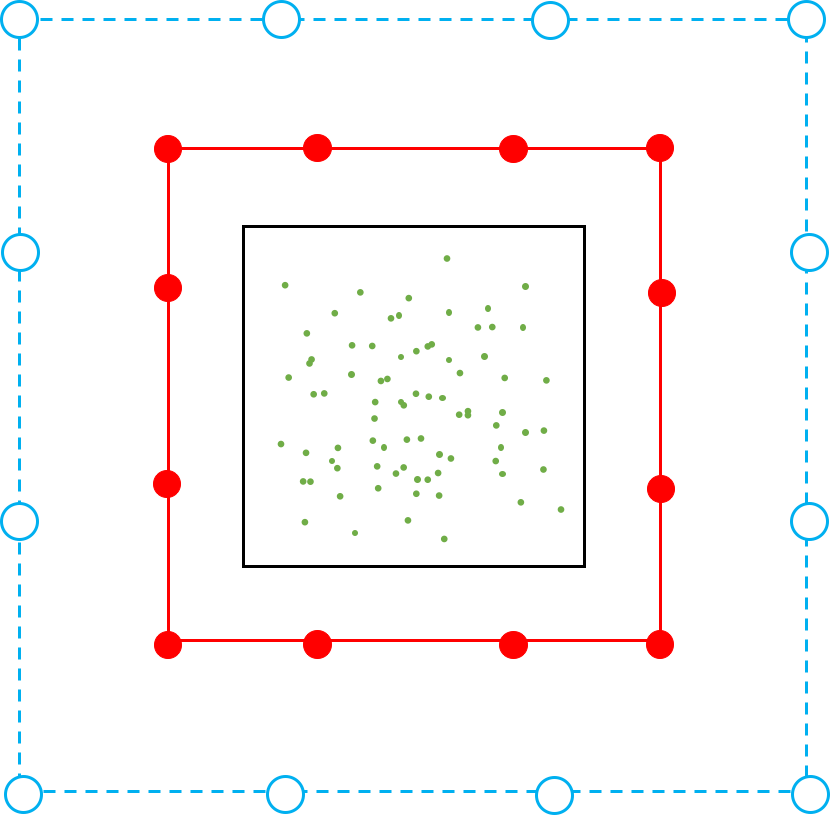
\includegraphics[width=0.3\textwidth]{introduction/upward_surface.png}}
    \hfill
  {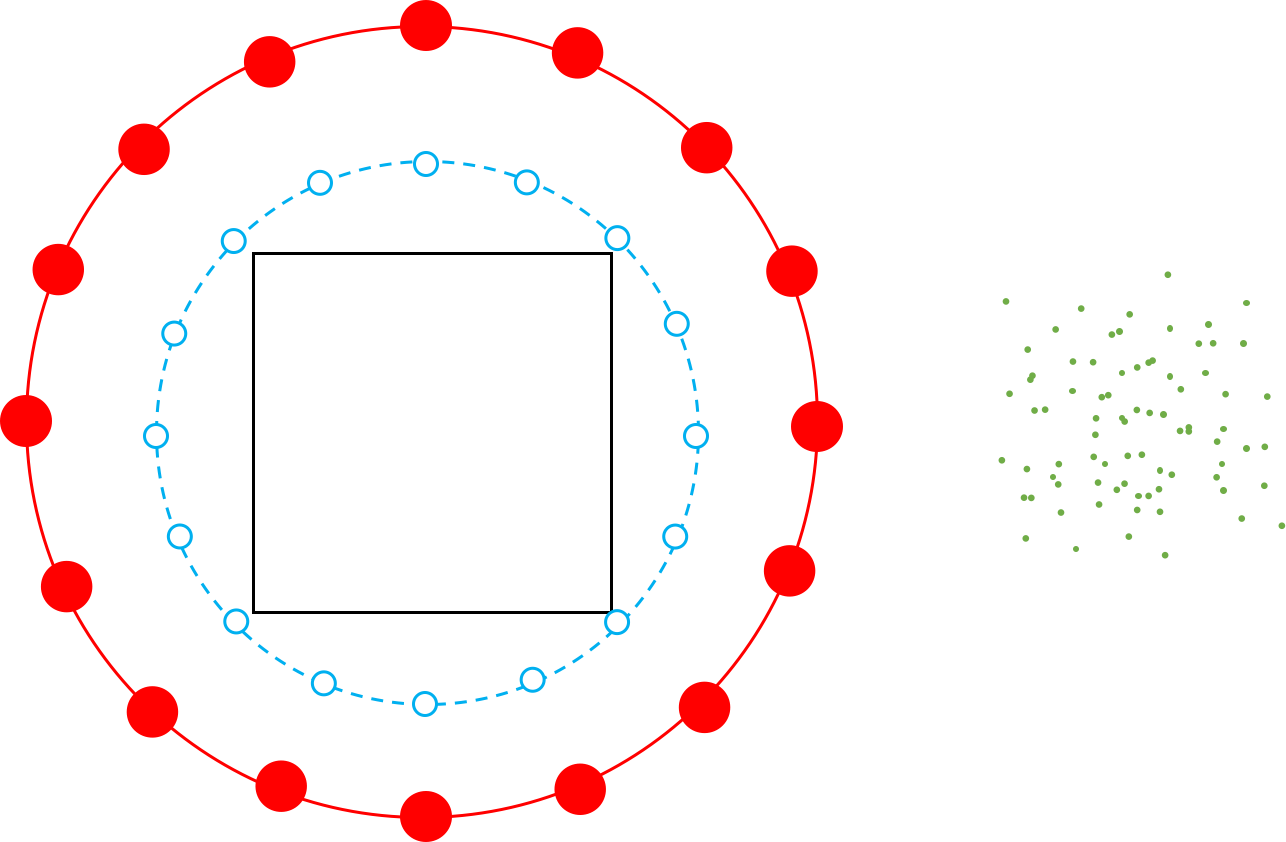
\includegraphics[width=0.4\textwidth]{introduction/downward_surface.png}}
  \vspace{0pt}
  \caption{Cross section of three dimensional cubic upward/downward equivalent and
    check surfaces. Source points are denoted by green circles. Red solid lines
    denote equivalent surfaces, and blue checked lines denote check surfaces. This
    figure is adapted directly from \cite{Ying:2004:JCP}.}
  \label{fig:1_2_upward_downward_surfaces}
\end{figure}

where we use the integral form of (\ref{eq:n_body_problem}) for the summation of
the contribution from the equivalent densities, and $q^{B, u}$ is referred to as
the \textbf{upward \gls{check-potential}}, with the other symbols taking their previous
definitions. We can define a very similar scheme for the case in which the source
densities are in $\mathcal{F}^B$, as a potential induced by a
\textbf{downward \gls{equivalent-density}} $\phi^{B,d}$ supported at discrete points
on a \textbf{downward \gls{equivalent-surface}} $\mathbf{y}^{B,d}$. This surface
needs to be located between the boundary of $\mathcal{F}^B$ and $B$, and again
as the solution for interior Dirichlet style problems for the types of PDEs we
consider is also unique \cite{Ying:2004:JCP}, we can equate the potentials generated
by the source points with that generated by the equivalent densities at some surface
between $\mathbf{y}^{B,d}$ and $B$. We call this surface the \textbf{downward \gls{check-surface}},
$\mathbf{x}^{B,d}$, and a corresponding mathematical statement of the equality of
the potentials can be written as follows,

\begin{equation}
    \int_{\mathbf{y}^{B,d}} K(\mathbf{x}, \mathbf{y})\phi^{B, d} d\mathbf{y} = \sum_{i \in I_s^{\mathcal{F}^B}} K(\mathbf{x}, \mathbf{y})\phi_i = q^{B, d} \> \> \text{for any} \> \> \mathbf{x} \in \mathbf{x}^{B, d}
    \label{eq:1_2_p2l}
\end{equation}

where $I_s^{\mathcal{F}^B}$ represents the indices of source points in the \gls{far-field}
of $B$, and $q^{B, d}$ is the \textbf{downward \gls{check-potential}}.

The equation (\ref{eq:1_2_p2m}) is an Fredholm integral
equation, of the first kind, and it's clear that its solution $\phi^{B, u}$
can be seen to be equivalent to the multipole expansion for the \gls{source-particles} contained in $B$. Therefore,
(\ref{eq:1_2_p2m}) can be seen to be correspond to the \gls{P2M}
operation. Similarly, the solution of (\ref{eq:1_2_p2l}) can be seen
to correspond to a particle-to-local, or P2L operation. Crucially, this method of solving
a set of linear equations to find equivalents of the multipole and local expansions
does not depend on finding a series expansion of a kernel function, and just on its evaluation.

Using this language of equivalent densities and check surfaces, we are also able to
write operations equivalent to the M2M, L2L and M2L operations. For a box $A$
and it's parent box $B$, the M2M operation can be written as,

\begin{equation}
    \int_{\mathbf{y}^{A,u}} K(\mathbf{x}, \mathbf{y})\phi^{A, u} d\mathbf{y} =   \int_{\mathbf{y}^{B,u}} K(\mathbf{x}, \mathbf{y})\phi^{B, u} d\mathbf{y}, \> \> \text{for any} \> \> \mathbf{x} \in \mathbf{x}^{B, u}
    \label{eq:1_2_m2m}
\end{equation}

Once $\phi^{A, u}$ has been calculated for boxes at the leaf level of the tree,
one can apply (\ref{eq:1_2_m2m}) to evaluate the multipole expansions for all
the boxes containing \gls{source-particles} in the tree in a manner equivalent
to the upward pass of Section \ref{sec:1_1_fmm_overview}. The M2M operation is
illustrated in figure (\ref{fig:1_2_m2m_l2l}A).

For the downward pass, the M2L operation, between a box $B$ and a box $A$ in its
interaction list can be written as,

\begin{equation}
    \int_{\mathbf{y}^{A,u}} K(\mathbf{x}, \mathbf{y})\phi^{A, u} d\mathbf{y} =   \int_{\mathbf{y}^{B,d}} K(\mathbf{x}, \mathbf{y})\phi^{B, d} d\mathbf{y}, \> \> \text{for any} \> \> \mathbf{x} \in \mathbf{x}^{B, d}
\label{eq:1_2_m2l}
\end{equation}

This is illustrated in figure (\ref{fig:1_2_m2l}). Once the local expansions
have  been computed starting at level 2 of the tree, we can perform the L2L
operation to transfer the local expansion of a parent box to its children,
for a box $A$ and it's child $B$, which can be written as,

\begin{equation}
    \int_{\mathbf{y}^{A,d}} K(\mathbf{x}, \mathbf{y})\phi^{A, d} d\mathbf{y} =   \int_{\mathbf{y}^{B,d}} K(\mathbf{x}, \mathbf{y})\phi^{B, d} d\mathbf{y}, \> \> \text{for any} \> \> \mathbf{x} \in \mathbf{x}^{B, d}
    \label{eq:1_2_l2l}
\end{equation}

\begin{figure}[!h]
    \centering
    {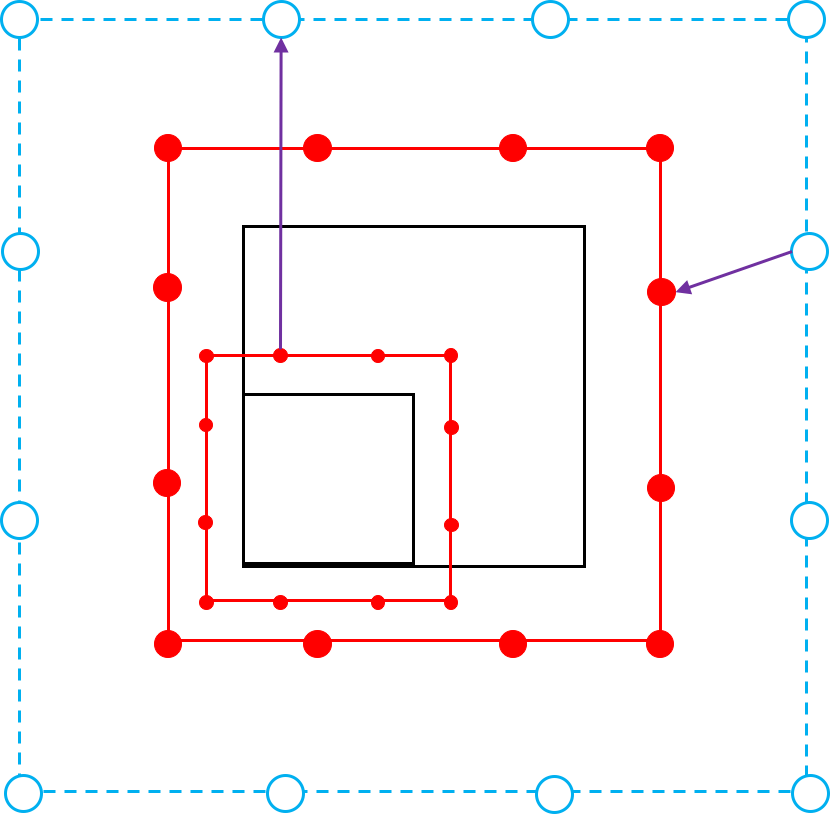
\includegraphics[width=0.4\textwidth]{introduction/kifmm_m2m.png}}
    \hfill
  {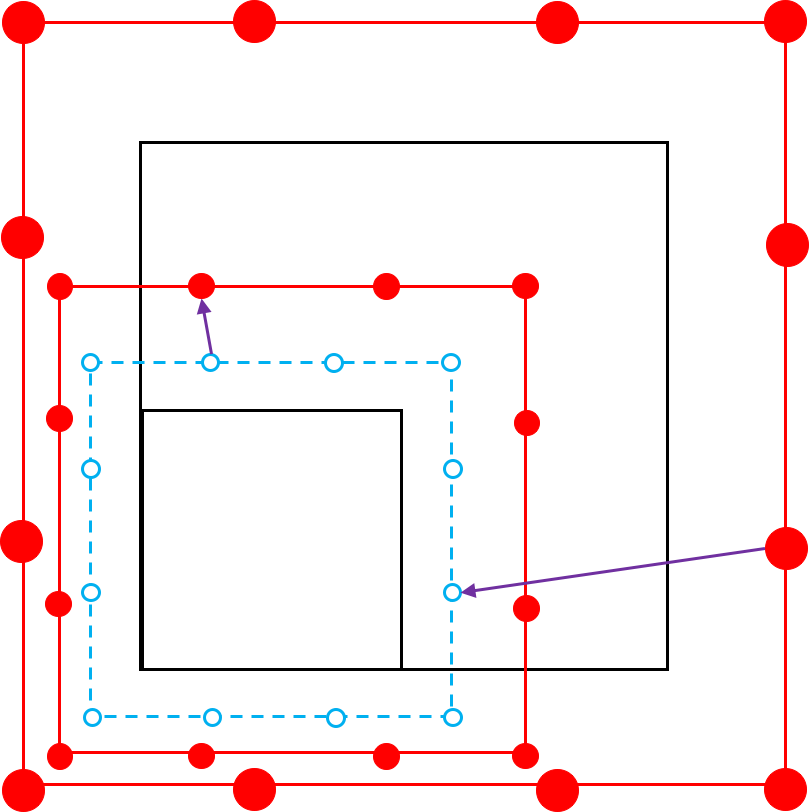
\includegraphics[width=0.4\textwidth]{introduction/kifmm_l2l.png}}
  \vspace{0pt}
  \caption{Cross section of three dimensional cubic surfaces. The (A) M2M operation and (B) L2L operation. Red solid lines
  denote equivalent surfaces, and blue checked lines denote check surfaces. This
  figure is adapted directly from \cite{Ying:2004:JCP}.}
  \label{fig:1_2_m2m_l2l}
\end{figure}

The M2M, L2L and M2L operations are illustrated using cubic surfaces in figure (\ref{fig:1_2_m2m_l2l})
The reason for using cubic check and equivalent surfaces are for ease of integration
in the case where the discretisation points chosen are from a regular Cartesian
grid.

\begin{figure}[!h]
    \centering
    {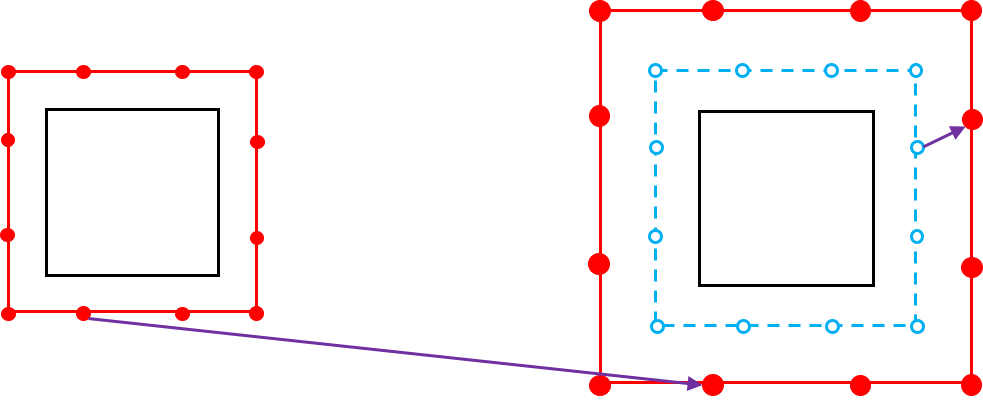
\includegraphics[width=\textwidth]{introduction/kifmm_m2l.png}}
    \caption{Cross section of three dimensional cubic surfaces for the M2L operation.}
  \label{fig:1_2_m2l}
\end{figure}

In principle, it is now possible to replace the kernel function expansions with
the appropriate solutions of the integral equations (\ref{eq:1_2_p2m}),
(\ref{eq:1_2_m2m}), (\ref{eq:1_2_l2l}) and (\ref{eq:1_2_m2l}). However all of
the above equations are ill-conditioned, as they are ill-posed and in general infinite
dimensional problems, and therefore require appropriate regularisation in order to solve.
Consider the following general statement of the first-kind Fredholm equation
that each of the above operations requires,

\begin{equation}
K \phi = q
\label{eq:1_2_first_kind_fredholm}
\end{equation}

We can use Tikhonov regularisation to write the solution,

\begin{equation}
\phi = (\alpha I + K^*K)^{-1}q
\end{equation}

where $\alpha$ is an appropriate regularisation parameter, and $I$ is the identity
matrix. This equation, a second-kind Fredholm equation, can be solved in numerous
ways. The authors of \cite{Ying:2004:JCP} make use of a Nystroem method, and indicate
the possibility of using either Galerkin or Collocation methods. For ease of
implementation, we choose instead to approximate the solution using a pseudo-inverse
estimated using a Singular Value Decomposition, or \textbf{\gls{SVD}}.

Consider the SVD of a matrix $A$, with $m$ rows and $n$ columns,

\begin{equation}
    A = U \Sigma V^*
\end{equation}

we can write an pseudo-inverse of $A$ as \cite{Trefethen:1997:SIAM},

\begin{equation}
    A^\dagger = V \Sigma U^*
\end{equation}

Furthermore, singular vectors corresponding to small singular values below a user
specified tolerance to increase the numerical stability of

\subsection{Summary}

